\chapter{Collaborative filtering}
\label{chp:03-recommendationSystems}
In questo capitolo verranno approfonditi gli algoritmi di raccomandazione implementati nella soluzione, mostrando le porzioni di 
codice e spiegando i vari passagi che portano ad ottenere delle raccomandazioni.
% - nel capitolo dei recommendation system parlare dei collaborative filter in modo più dettagliato e legato al progetto -


\section{Memory-based} 
I Filtri Collaborativi Memory-based sono stati introdotti per via delle osservazioni e studi dimostrando che
gli utenti si fidano maggiormente delle raccomandazioni di altri che la pensano allo stesso modo. Questi metodi mirano a determinare 
il grado o il tipo di relazione tra utenti e item identificando o coppie di item che tendono ad essere usati insieme 
o che hanno un grado di similarità alto oppure utenti con uno storico di item usati simile
\cite{taxonomy-of-recommender-agents-on-the-internet}.
Questi approcci divennero molto famosi grazie alla loro semplicità di implementazione, molto intuitivi, non necessitano di operazioni
di training sui dati e regolazione di molti parametri, inoltre l'utente può comprendere la ragione che si cela dietro
ad ogni raccomandazione. 

Questa categoria di sistemi di raccomandazione è definita anche \\\textit{Neighborhood-based} e può essere ulteriormente 
classificata in due sottocategorie:


\subsection{User-based filtering} 
Questo sistema, definito anche con l'acronimo UB-CF (\textit{User-based Collaborative Filter}), basa tutto il suo funzionamento sulla 
comunità di utenti, maggiore è la sua dimensione e l'attività degli utenti con item o servizi e migliori potranno essere le 
raccomandazioni. Questo algoritmo fornisce dei suggerimenti ad un utente sulla base di uno o più vicini (neighbours), e la similarità 
tra utenti può essere determinata sulla base degli item che l'utente ha utilizzato o valutato.

Molti di questi approcci possono essere generalizzati dall'algoritmo organizzato nei seguenti passi:
\begin{enumerate}
	\item Specificare qual'è l'utente a cui si vuole applicare l'algoritmo di raccomandazione e recuperare quali utenti possono 
	avere dato valutazioni o usato item simili al utente target. Piuttosto che recuperare tutti gli utenti, per velocizzare l'esecuzione
	dell'algoritmo, è possibile selezionare soltanto un gruppo di utenti in modo casuale oppure associare dei valori di similarità tra 
	tutti gli utenti e confrontando questi valori con quello dell'utente target, selezionare i relativi utenti che superano una soglia
	scelta, oppure utilizzare tecniche di clustering.
	\item Estrarre quegli item a cui l'utente target non ha mai interagito e per questo motivo gli possono interessare, e mostrarli 
	sottoforma di raccomandazioni.
\end{enumerate}

\begin{figure}[ht!]
	\centering
	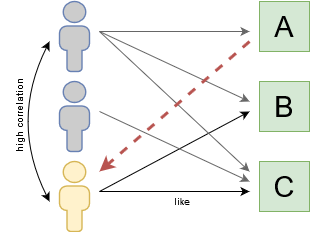
\includegraphics[scale=0.5]{images/UB_CF_ex.png}
	\caption{Esempio di applicazione di un sistema di raccomandazione User-based}
	\label{fig:UB_CF}
\end{figure}
\ \\
Questi approcci sono facilmente implementabili, indipendenti dal contesto in cui sono applicati e possono essere più accurati rispetto
a tecniche basate sul Content-based filtering; dall'altra parte all'aumentare del numero di utenti che vado a considerare per fare le 
raccomandazioni migliore è la precisione di questo processo ma anche è maggiore il costo in termini di tempo.\\  

Nella soluzione proposta in questa tesi, l'algoritmo UB-CF viene implementato come funzione che prende in ingresso un parametro 
\textit{user\_other\_id}, come è possibile osservare dal Codice \ref{lst:UB_CF_1} corrispondente all'identificativo dell'utente, 
e restituisce una lista di raccomandazioni \textit{similar\_user\_evaluations} corrispondenti alle Evaluation simili a quelle usate 
da altri utenti. 
\lstset{style=python_code_style}
\begin{lstlisting}[language=Python, label=lst:UB_CF_1, caption={\ }]
# User recommendation algortihm
def user_recommendation_alg(user_other_id):
\end{lstlisting}
\ \\
Più precisamente il funzionamento dell'algoritmo si svolge seguendo i seguenti passi:
\begin{itemize}
	\item il primo passo è quello di recuperare sulla base del parametro in ingresso alla funzione, lo \textit{user\_other\_id},
	tutte le Evaluation utilizzate dall'utente in questione
	\begin{lstlisting}[language=Python, label=lst:UB_CF_2]
		# Select the target user and its evaluations
		target_user_evaluations = User.objects.get(other_id=user_other_id).evaluations.all()\
																					.values('other_id', 'id', 'parent_id')\
																					.order_by('other_id')
	\end{lstlisting}
	\item il secondo passo consiste nel selezionare le Evaluation usate dagli altri utenti, e creare una lista di queste Evaluation
	\textit{other\_users\_evaluations};
	\begin{lstlisting}[language=Python, label=lst:UB_CF_3]
		# Select all other users and theirs evaluations
		other_users = User.objects.exclude(other_id=user_other_id)
		# Creating a list with all the evaluations of other users
		other_users_evaluations = []
		for o_users_evaluation in other_users:
			for evaluation in o_users_evaluation.evaluations.all().values('other_id', 'id', 'parent_id')\
																	.order_by('other_id'):
				other_users_evaluations.append(evaluation)
	\end{lstlisting}
	\item il terzo passo consiste nell'andare a determinare quali tra le Evaluation, dell'utente a cui si vuole raccomandare, quali sono quelle 
	simili usate dagli altri utenti. Per determinare le Evaluation simili si è andato a confrontare il paramentro \textit{parent\_id} (che identifica
	all'interno della base di dati quale sia il nodo padre per quella Evaluation), associato ad ogni Evaluation, in questo modo si è andati a selezionare
	soltanto gli item appartenenti a una stessa categoria, inoltre vengono eliminanti eventuali nodi duplicati. E componendo una lista finale 
	\textit{similar\_user\_evaluations} con le Evaluation restanti. 
	In definitiva ciò che ritorna questa funzione sono due liste: \textit{target\_user\_evaluations}, contenente le Evaluation usate dall'utente 
	in questione e \textit{similar\_user\_evaluations}.
	\begin{lstlisting}[language=Python, label=lst:UB_CF_4]
		# Comparing target user's evaluations and other user's evaluations, and if there is a match the evaluation is
		# added to the 'similar_evaluations' list (the matching is made comparing the 'parent_id')
		similar_user_evaluations = []
		for t_user_evaluation in target_user_evaluations:
			for o_users_evaluation in other_users_evaluations:
				# Taking only the evaluations that have: different other_id (excluding the target evaluation
				# in the recommendation) and same parent_id and the evaluations that weren't added to 'target_user_evaluations'
				# list and to 'similar_user_evaluations'
				if ((t_user_evaluation['other_id'] != o_users_evaluation['other_id']) and  # Evaluations must have different 'other_id'
						(t_user_evaluation['parent_id'] == o_users_evaluation['parent_id']) and  # Evaluations must have the same 'parent_id'
						# Evaluation in all_other_evals list mustn't be already added to \
						not (o_users_evaluation in target_user_evaluations) and  # the 'target_user_evaluations' list or
						not (o_users_evaluation in similar_user_evaluations)):  # the 'similar_user_evaluations' list
					similar_user_evaluations.append(o_users_evaluation)
					
    	return target_user_evaluations, similar_user_evaluations
	\end{lstlisting}
\end{itemize}

%% ESEMPIO DI UNA CHIAMATA CON VALORE DI RITORNO
%\begin{figure}[ht!]
%	\centering
%	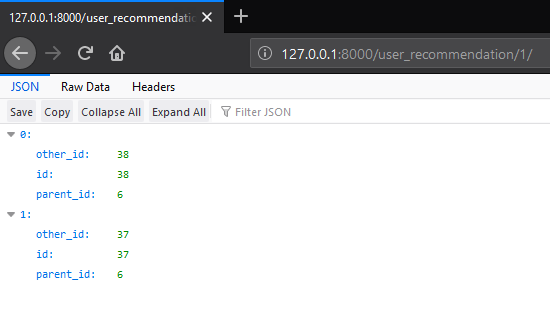
\includegraphics[scale=0.5]{images/UB_CF_test.png}
%	\caption{Esempio di esempio di una risposta in JSON a una chiamata Rest all'algoritmo di raccomandazione UB-CF.}
%	\label{fig:UB_CF_resp_json}
%\end{figure}
\ \\
Nel capitolo successivo verrano mostrati degli esempi pratici in cui è stato applicato questo algoritmo.

\newpage

\subsection{Item-based filtering} 
Quando viene applicato per milioni di utenti e item l'algoritmo UB-CF non è molto efficente per via della complessa computazione della 
ricerca di utenti simili; così in alternativa è stato introdotto l'algoritmo di Filtraggio Item-based, definito anche IB-CF 
(\textit{Item-based Collaborative Filter}) dove piuttosto che effetuare il confronto tra utenti simili, viene fatto un confronto tra 
gli item dell'utente a cui si vuole raccomandare e i possibili item simili.

\begin{figure}[ht!]
	\centering
	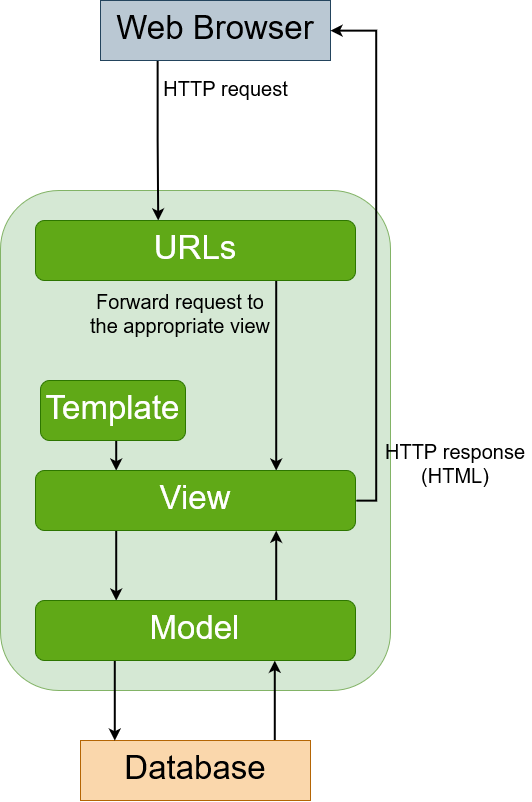
\includegraphics[scale=0.5]{images/IB_CF_ex.png}
	\caption{Esempio di applicazione di un sistema di raccomandazione IB-CF.}
	\label{fig:IB_CF}
\end{figure}
\ \\
Questi sistemi sono estremamente simili ai sistemi di raccomandazione Content-based, e identificano item simili in base a come sono
stati usati dagli utenti in passato \cite{item-based-collaborative-filtering}.

A livello pratico nella soluzione proposta, questo algoritmo è stato implementato come funzione che prende in ingresso un 
parametro \textit{item\_other\_id} rappresentante l'\textit{other\_id}, un attributo associato ad ogni item all'interno della base di dati
che lo identifica, del item su cui si vuole ottenere altri item simili; in generale per determinare la similarità tra due oggetti, si osserva 
l'attributo \textit{parent\_id} associato ad ogni item, che determina quale sia il nodo padre all'interno della tassonomia, in sostanza 
vengono selezionati quegli item che appartengono alla stessa categoria.\\

In generale il CF-IB ideato per determinare Evaluation simili funziona seguendo i seguenti passi:
\begin{itemize}
	\item il primo passo è quello di recuperare sulla base del parametro in ingresso alla funzione (item\_other\_id)
	l'Evaluation su cui si vuole determinare le altre Evaluation simili;
	\begin{lstlisting}[language=Python, label=lst:IB_CF_Evaluation_1]
	def item_recommendation_alg(item_other_id):

		# Selecting the evaluation, which is applied this algorithm, from its other_id
		# SELECT * FROM recommendation_app_evaluation WHERE other_id = %(item_other_id)s AND node_type = 'eva'
		target_eval = Evaluation.objects.filter(Q(other_id=item_other_id) & Q(node_type="eva"))\
										.values('other_id', 'id', 'parent_id')[0]
	\end{lstlisting} 
	\item il secondo passo è quello di recuperare tutte le Evaluation, escludendo la prima recuperata, presenti nella base di dati;
	\begin{lstlisting}[language=Python, label=lst:IB_CF_Evaluation_2]
		# Selecting the other evaluations, excluding the target evaluation
		# SELECT * FROM recommendation_app_evaluation WHERE other_id != %(item_other_id)s AND node_type = 'eva'
		all_other_evals = Evaluation.objects.filter(~Q(other_id=item_other_id) & Q(node_type="eva"))\
											.values('other_id', 'id', 'parent_id').order_by('other_id')
	\end{lstlisting}
	\item il terzo ed ultimo passo consiste nel andare a determinare le Evaluation che hanno lo stesso parent\_id, quindi
	quelle appartenenti alla stessa categoria, dell'Evaluation ottenuta nel primo passo; inoltre, se presenti, vengono 
	eliminati eventuali duplicati; e la funzione ritorna una lista \textit{similar\_item\_evaluations} contente le Evaluation simili.
	\begin{lstlisting}[language=Python, label=lst:IB_CF_Evaluation_3]
		# Creating a list with all the evaluations that are similar to the target evaluation (comparing the parent_id)
		similar_item_evaluations = []
		for evaluation in all_other_evals:
			# Taking only the evaluations that have: different other_id (excluding the target evaluation
			# in the recommendation) and same parent_id and the evaluations that weren't added to similar_item_evaluations
			# list
			if ((target_eval['other_id'] != evaluation['other_id']) and  # Evaluations must have different 'other_id'
					(target_eval['parent_id'] == evaluation['parent_id']) and  # Evaluations must have same 'parent_id'
					# Evaluation in all_other_evals list mustn't be already added to \
					not (evaluation in similar_item_evaluations)): # the 'similar_item_evaluations' list
				similar_item_evaluations.append(evaluation)

	return similar_item_evaluations	
	\end{lstlisting}
\end{itemize}

%% ESEMPIO DI UNA CHIAMATA
%\begin{figure}[ht!]
%	\centering
%	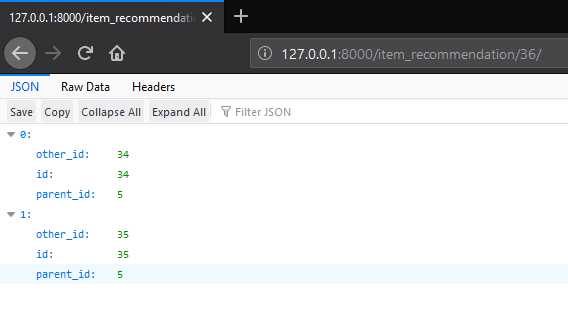
\includegraphics[scale=0.5]{images/IB_CF_Evaluation_test.png}
%	\caption{Esempio di esempio di una risposta in JSON a una chiamata Rest all'algoritmo di raccomandazione IB-CF per le Evaluation
%	supportate da Moon Cloud.}
%	\label{fig:IB_CF_Eval_resp_json}
%\end{figure}
\ \\
Altro algoritmo del tipo IB-CF implementato in questa tesi sulla falsa riga di quello appena riportato qua sopra, è quello ideato per
determinare quali Evaluation possono essere raccomandate per un Target inserito da un utente tra quelli supportati da Moon Cloud,
che sono: Host avente Windows come sistema operativo, Host avente Linux come sistema operativo, sistemi che sfruttano 
servizi di Aws o di Azure e Url di siti web.\\
In Python questo algoritmo viene implementato come funzione che prende in ingresso l'\textit{id} (identificativo univoco) del Target, e 
restituisce l'insieme delle Evaluation raccomandate per quel Target; il tutto viene eseguito seguendo questi passi:
\begin{itemize}
	\item il primo passo è quello di recuperare tutte le Evaluation presenti nel database;
	\begin{lstlisting}[language=Python, label=lst:IB_CF_Target_1]
	def target_recommendation_alg(target_id):
		# Retriving all the evaluations in the database
		evaluations = Evaluation.objects.filter(node_type="eva")
	\end{lstlisting} 
	\item il secondo ed ultimo passo è quello di andare a determinare quali sono i Controlli che hanno il valore dell'attributo \textit{target\_type\_id}
	pari al parametro in ingresso della funzione \textit{target\_id}, e da quei Controlli determinare le Evaluation che li utilizzano, 
	eliminando eventuali duplicati; determinando così le possibili Evaluation applicabili per quel Target.
	\begin{lstlisting}[language=Python, label=lst:IB_CF_Target_2]
		# Saving in the target_evaluations list the evaluations which controls have target_type_id equal to target_id
		target_evaluations = []
		for evaluation in evaluations: # Scanning all the evaluations
			for evaluation_controls in evaluation.controls.filter(target_type_id=target_id):
				if not(evaluation in target_evaluations): # Excluding evaluations duplicated
					target_evaluations.append(evaluation)
	
		# Converting the Evaluation model's instance in a dict and putting the evaluation, as a dict, in a list
		target_evaluations_serializer = EvaluationSerializer(target_evaluations, many=True)

		return target_evaluations_serializer.data
	\end{lstlisting} 
\end{itemize}

%% ESEMPIO DI UNA CHIAMATA
%\begin{figure}[ht!]
%	\centering
%	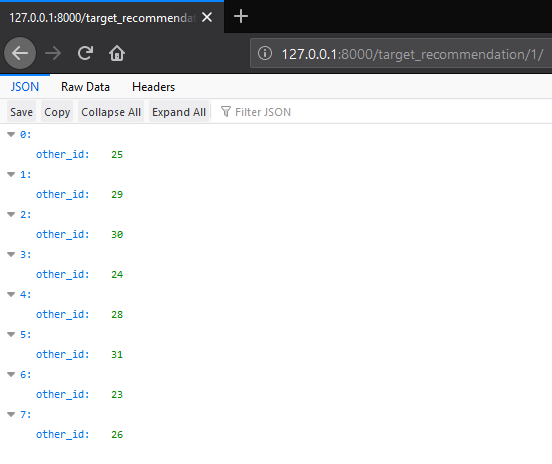
\includegraphics[scale=0.5]{images/IB_CF_Target_test.png}
%	\caption{Esempio di esempio di una risposta in JSON a una chiamata Rest all'algoritmo di raccomandazione IB-CF per i 
%	Target supportarti da Moon Cloud.}
%	\label{fig:IB_CF_Target_resp_json}
%\end{figure}
\ \\
Nel capitolo successivo verrano mostrati anche degli esempi dei valori di risposta di queste funzioni.

\subsection{Hybrid filtering} 
Nei sistemi di raccomandazione ibridi si tende a voler combinare più tecniche di raccomandazione, cercando di raggruppare i 
pregi di ciascuna tecnica; infatti se uno compara i sistemi di raccomandazione ibridi con i sistemi Collaborativi o 
Content-based, la precisione dei suggerimenti è solitamente maggiore.\\
Nella soluzione proposta in questa tesi, questo algoritmo viene direttamente implementato come Api Rest, alla quale viene 
passato come parametri la request, l'oggetto HTTP che il browser invia al server contenente la richiesta HTTP attraverso
un certo URL e lo user\_other\_id è un valore che viene preso dall'URL, e rappresenta l'other\_id dell'utente su cui si andrà
a raccomandare. Inoltre il tutto viene limitato ad essere richiamato solo tramite richieste HTTP con metodo GET.\\ 
Nel codice \ref{lst:CF_Hybrid_Evaluation_1} possiamo vedere come vengono limitate le richieste al metodo GET e come 
viene definita la funzione.

\begin{lstlisting}[language=Python, label=lst:CF_Hybrid_Evaluation_1, caption={\ }]
@api_view(['GET'])
def hybrid_recommendation(request, user_other_id)
\end{lstlisting} 
\ \\
Il funzionamento di questo algoritmo si svolge nei seguenti passi:
\begin{itemize}
	\item il primo passo è quello di verificare se l'utente esiste nel database altrimenti viene generata un eccezione (errore) che viene gestito in
	modo personalizzato, generando una risposta HTTP con codice di errore 404 (Not Found);
	\begin{lstlisting}[language=Python, label=lst:CF_Hybrid_Evaluation_2]
		# Trying to retrive the actual User with user_other_id
		user = User.objects.get(other_id=user_other_id)
	\end{lstlisting} 
	\item il secondo passo è applicare l'algoritmo di User Recommandation, descritto nella sezione precendete, per le Evaluation e ottenere due liste,
	la prima target\_user\_evaluations contiene le Evaluation che l'utente ha utilizzato, mentre nella seconda similar\_user\_evaluations si avranno
	le Evaluation che gli altri utenti hanno utilizzato e che sono simili alle Evaluation del primo utente;
	\begin{lstlisting}[language=Python, label=lst:CF_Hybrid_Evaluation_3]
		# Taking from the user_recommendation_alg the evaluation recommended from this approach (similar_user_evaluations)
		# and the user's evaluations (target_user_evaluations)
		target_user_evaluations, similar_user_evaluations = user_recommendation_alg(user_other_id)
	\end{lstlisting} 
	\item il terzo passo consiste nell'applicazione dell'algoritmo Item-based per ogni Evaluation usata dall'utente in questione così da ottenere 
	delle raccomandazioni che sono compatibili con le Evaluation usate dall'Utente; la similarità o appartenenza alla stessa categoria viene 
	ottenuta osservando il valore del parent\_id; anche in questo caso vengono eliminati eventuali duplicati e viene formata una lista 
	similar\_item\_evaluations contenente le Evaluation simili ottenute dall'applicazione dell'algoritmo di raccomandazione Item-based;
	\begin{lstlisting}[language=Python, label=lst:CF_Hybrid_Evaluation_4]
		# For every evaluation used by users is extracted all other possible evaluations that have the same 'parent_id'
		similar_item_evaluations = []
		for t_user_evaluation in target_user_evaluations:  # for every target user's evaluations
			for item_evaluation in item_recommendation_alg(t_user_evaluation['other_id']):  # is applied the item_recommendation algorithm
				# Taking only the evaluations that have: different other_id (excluding the target evaluation
				# in the recommendation) and same parent_id and the evaluations that weren't added to 'similar_item_evaluations'
				# list or to 'similar_user_evaluations' or to 'target_user_evaluations'
				if ((t_user_evaluation['other_id'] != item_evaluation['other_id']) and # Evaluations must have different 'id'
						(t_user_evaluation['parent_id'] == item_evaluation['parent_id']) and # Evaluations must have the same 'parent_id'
						# Evaluation in all_other_evals list mustn't be already added to \
						not (item_evaluation in similar_item_evaluations) and # the 'similar_item_evaluations' list,
						not (item_evaluation in similar_user_evaluations) and # the 'similar_user_evaluations' list or
						not (item_evaluation in target_user_evaluations)): # the 'target_user_evaluations' list
					similar_item_evaluations.append(item_evaluation)
	\end{lstlisting} 
	\item il quarto passo consiste nel raggruppare le due liste contenenti le Evaluation raccomandate per l'utente secondo l'applicazione dei
	due algoritmi, eliminando anche eventuali duplicati, così da ottenere un'unica lista similar\_evaluations la quale viene ritornata dalla 
	funzione sottoforma di risposta HTTP in formato Json;
	\begin{lstlisting}[language=Python, label=lst:CF_Hybrid_Evaluation_5]
		# Putting together the evaluations recommended in similar_user_evaluations list and similar_item_evaluations list
		similar_evaluations = []
		# Adding to similar_evaluations list the evaluation in the similar_user_evaluations list
		for s_user_evaluation in similar_user_evaluations:
			similar_evaluations.append(s_user_evaluation)
		# Adding to similar_evaluations list the evaluation in the similar_item_evaluations list
		for item_evaluation in similar_item_evaluations:
			# Taking only the evaluations that weren't added to \
			if (not (item_evaluation in similar_evaluations) and # the 'similar_evaluations' list or
					not (item_evaluation in target_user_evaluations)): # the 'target_user_evaluations' list
				similar_evaluations.append(item_evaluation)
		similar_evaluations = sorted(similar_evaluations, key=lambda i: i['other_id'])

		return JsonResponse(similar_evaluations, safe=False)
	\end{lstlisting} 
\end{itemize}
\ \\
Nel capitolo successivo verrà mostrato un esempio di risposta quando viene chiamata questa funzione, e verrà approfondito il contesto che 
è stato costruito attorno agli algoritmi di raccomandazione descritti in questo capitolo.

%% ESEMPIO DI UNA CHIAMATA
%\begin{figure}[ht!]
%	\centering
%	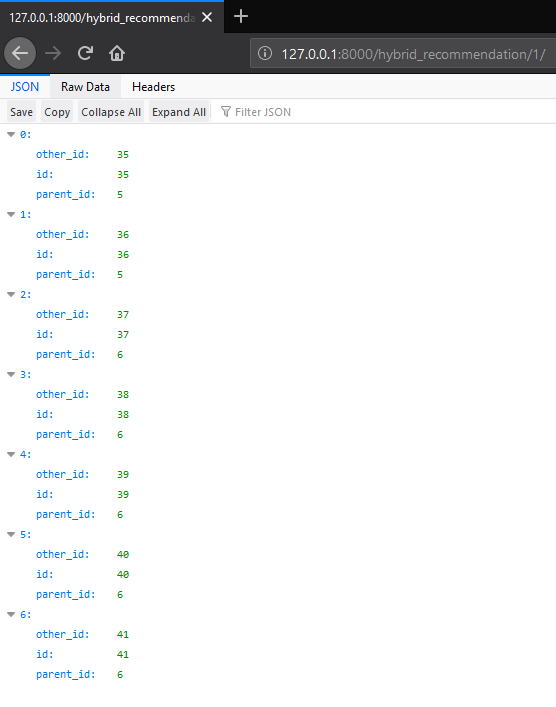
\includegraphics[scale=0.5]{images/CF_Hybrid_test.png}
%	\caption{Esempio di esempio di una risposta in JSON a una chiamata Rest all'algoritmo di raccomandazione Ibrido.}
%	\label{fig:CF_Hybrid_resp_json}
%\end{figure}